\documentclass[../main.tex]{subfiles}
\begin{document}

\section{Pick and Place Execution} \label{sec:robotics}
In this section, the robotics part of the pick and place solution is covered. Firstly in Section \ref{subsec:workcell_design}, the design of the workcell is described. Secondly in Section \ref{subsec:robot_motion_planning}, three algorithms for executing the pick and place action are described. The three algorithms are point to point interpolation, point to point interpolation with parabolic blend and rapidly-exploring random tree connect. The three algorithms will be evaluated and compared, and the best performing algorithm will be chosen to be used in the combination of robotics and vision in Section \ref{sec:combination}. 

\subsection{The Design of the Workcell} \label{subsec:workcell_design}
In this section, the reachability of the manipulator on the robot will be analyzed, by placing the robot base at different positions on the table. The table is shown in Figures \ref{subfig:table_areas} and \ref{subfig:placement_of_cylinders}. The manipulator must be able to reach the object at every position in the picking area, and then place the object in the center of the place area with as many collision free kinematic configurations as possible. In Figure \ref{subfig:table_areas} the picking and place areas are shown. To perform the reachability analysis the scene shown in Figure \ref{subfig:placement_of_cylinders} is used, the three different placements for picking and placing are shown here and the object used for the analysis. The positions of the cylinders in the picking area are chosen because these are the extremes.
\begin{figure}[H]
    \centering
    \begin{subfigure}[b]{0.49\textwidth}
        \centering
        \captionsetup{width=0.55\textwidth}
        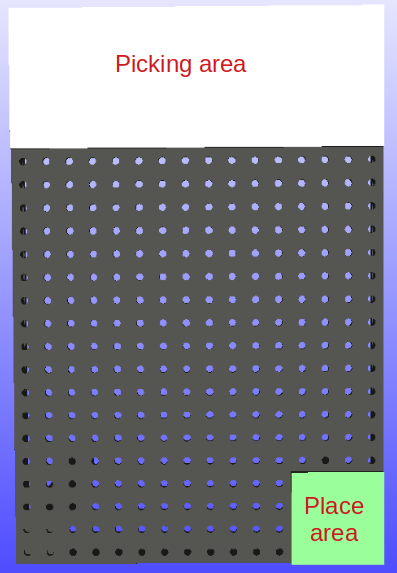
\includegraphics[width=0.55\textwidth]{figures/workcell_setup/pick_and_place.png}
        \caption{Illustration of the picking and place areas on the table.}
        \label{subfig:table_areas}
    \end{subfigure}
    \begin{subfigure}[b]{0.49\textwidth}
        \centering
        \captionsetup{width=0.9\textwidth}
        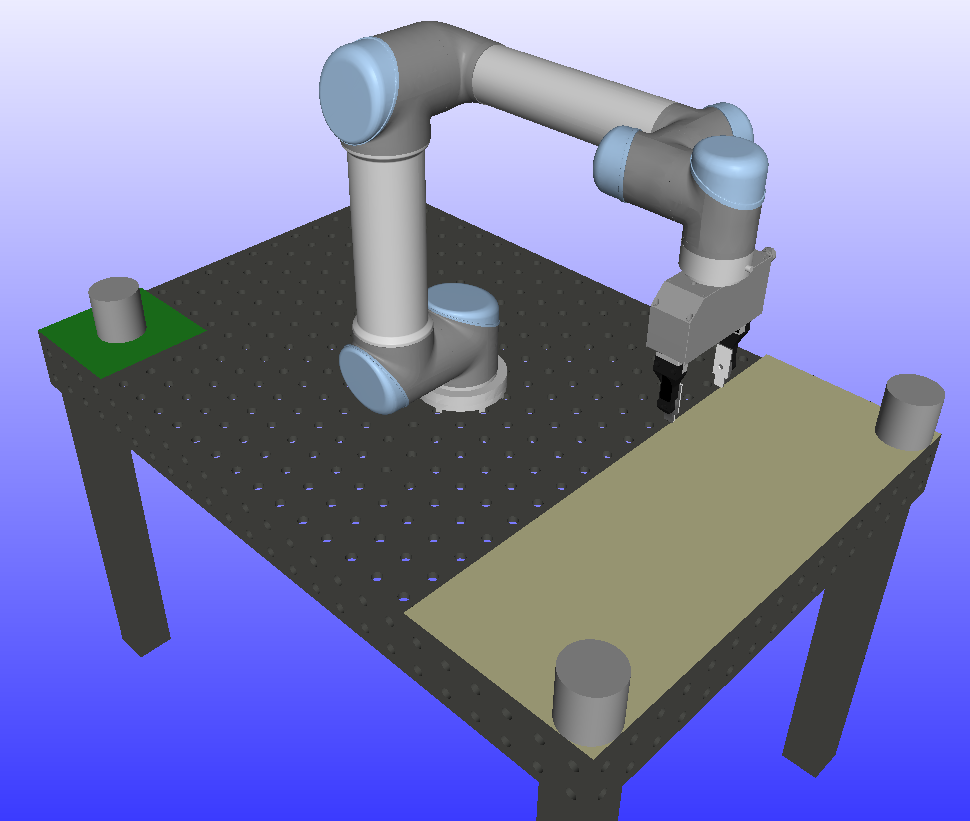
\includegraphics[width=0.9\textwidth]{figures/workcell_setup/placement_of_cylinders.png}
        \caption{Illustration of the placement of the cylinders and the initial placement of the robot base.}
        \label{subfig:placement_of_cylinders}
    \end{subfigure}
    \caption{Illustrations of the table for the reachability analysis.}
    \label{fig:table}
\end{figure}
In the reachability analysis two grasp configurations are considered: grasping from the side and grasping from the top. The grasp configurations are shown in Figure \ref{fig:close2singularities}, where the right most figure shows grasping from the top and the other two show grasping from the side. Figure \ref{fig:close2singularities} also shows three bad positions of the robot base, because the robot is close to singularities. Singularities are to be avoided, because of the high joint velocities resulting from passing close to them. 
\begin{figure}[H]
    \centering
    \begin{subfigure}{0.329\textwidth}
        \centering
        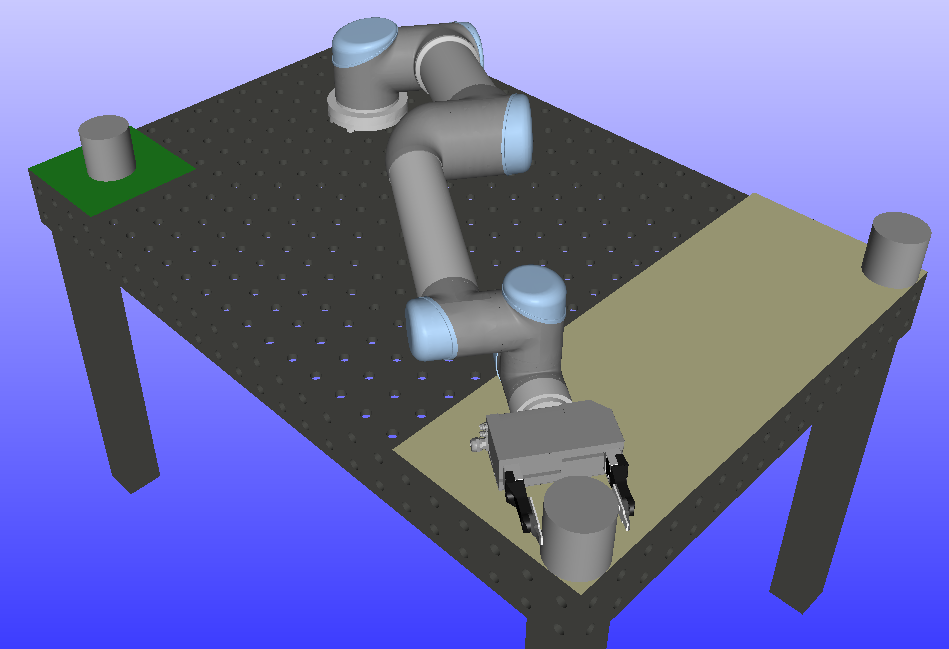
\includegraphics[width=0.9\textwidth]{figures/workcell_setup/singularity1.png}
    \end{subfigure}%
    \begin{subfigure}{0.329\textwidth}
        \centering
        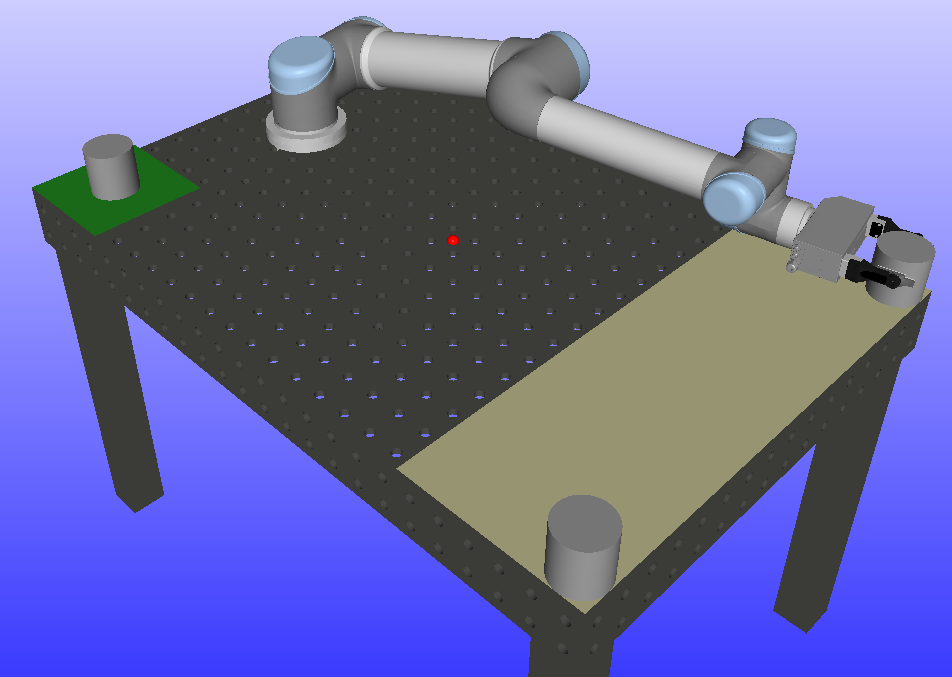
\includegraphics[width=0.9\textwidth]{figures/workcell_setup/singularity2.png}
    \end{subfigure}%
    \begin{subfigure}{0.329\textwidth}
        \centering
        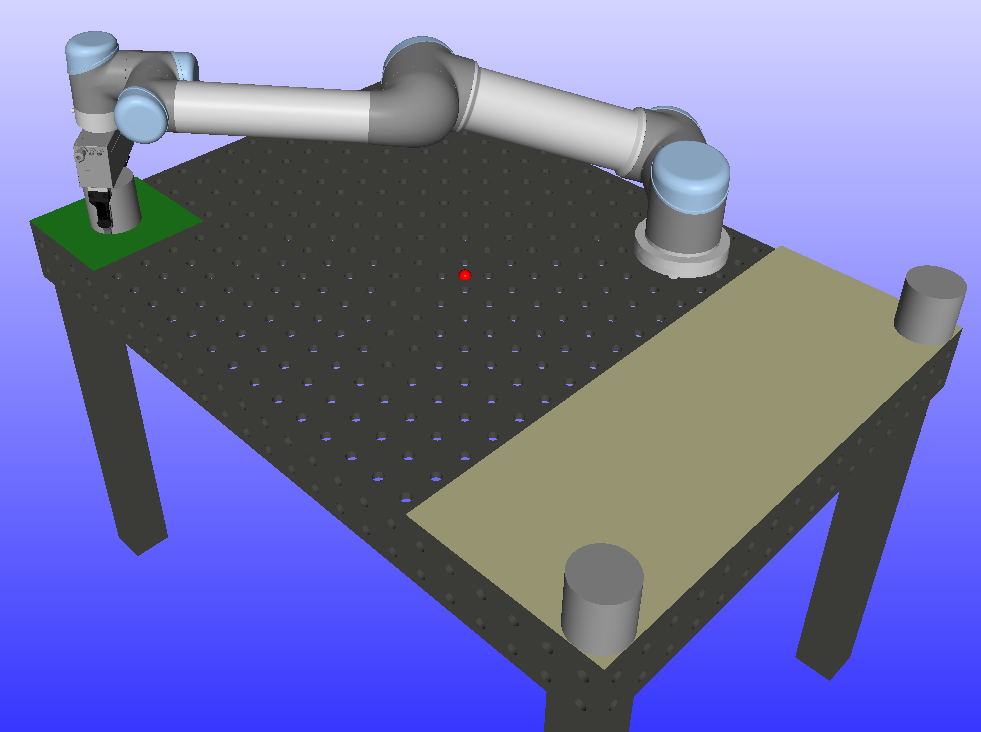
\includegraphics[width=0.9\textwidth]{figures/workcell_setup/singularity3.png}
    \end{subfigure}
    \caption{Illustrations of robot base positions which come close to singularities.}
    \label{fig:close2singularities}
\end{figure}
The almost singularity in Figure \ref{fig:close2singularities} is the elbow singularity, where joint two, three and four are coplanar. Other singularities which can occur are a wrist singularity and a shoulder singularity.

\textbf{Grasping from the side:}\\
The results from the reachability analysis when grasping from the side are illustrated in Figure \ref{fig:scatter_cylinder_side}. 

\begin{figure}[H]
    \centering
    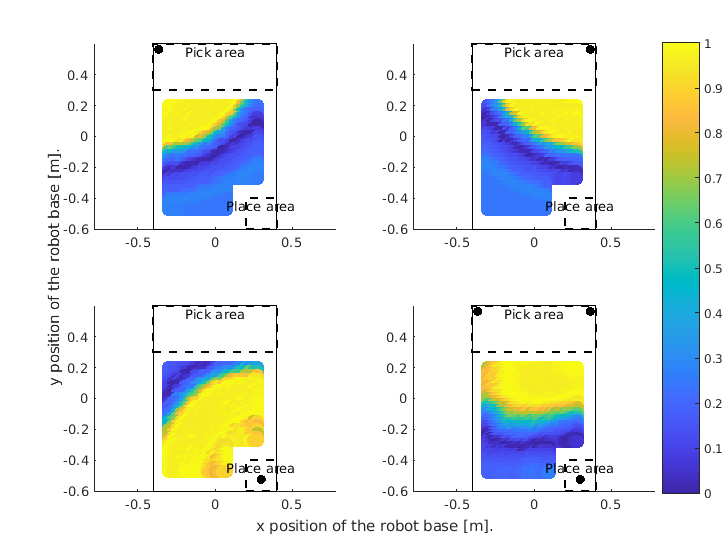
\includegraphics[width=0.8\textwidth]{figures/workcell_setup/scatter_cylinder_side.png}
    \caption{Scatter plots of the robot arm's ability to grasp a cylinder approaching from the side. The black circle indicates the cylinder position. The color scale indicates collision free kinematic solutions for the robot arm.}
    \label{fig:scatter_cylinder_side}
\end{figure}

In Figure \ref{fig:scatter_cylinder_side}, the cylinder position is illustrated as a black circle in the pick and place area. The color scale at the right of the figure indicates collision free kinematic solutions, e.g. a value of 1 means the manipulator can reach the cylinder from all $360$ degrees. The bottom right figure shows a combination of all cylinder positions, which indicates a good position of the robot base at the top half.

\textbf{Grasping from the top:}\\
The results from the reachability analysis when grasping from the top are illustrated in Figure \ref{fig:scatter_cylinder_top}.

\begin{figure}[H]
    \centering
    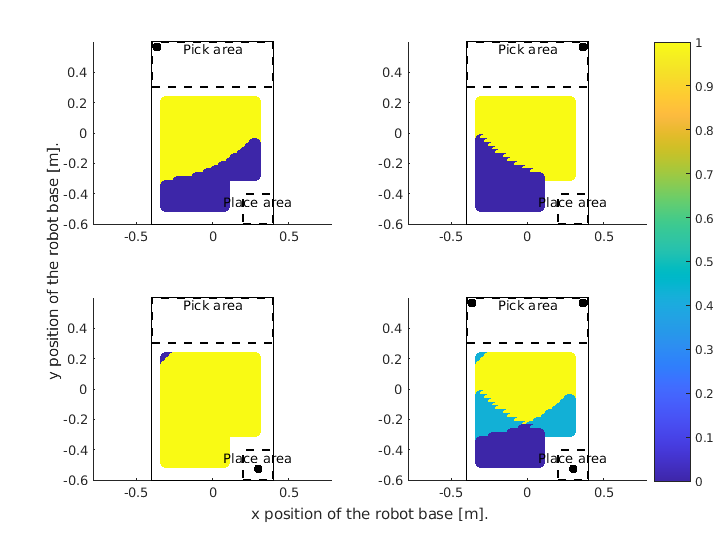
\includegraphics[width=0.8\textwidth]{figures/workcell_setup/scatter_cylinder_top.png}
    \caption{Scatter plots of the robot arm's ability to grasp a cylinder approaching from the top. The black circle indicates the cylinder position. The color scale indicates collision free kinematic solutions for the cylinders.}
    \label{fig:scatter_cylinder_top}
\end{figure}

The bottom right figure in Figure \ref{fig:scatter_cylinder_top} indicates a good position of the robot base at the half of the table near the picking area. 

Based upon the two reachability analyses, grasping from the side and grasping from the top, the best position of the robot base is at the half closest to the picking area. The robot base is placed at $(0.2, 0.0)$ on the table, which is illustrated in Figure \ref{fig:final_robot_position}.

\begin{figure}[H]
    \centering
    \begin{subfigure}{0.329\textwidth}
        \centering
        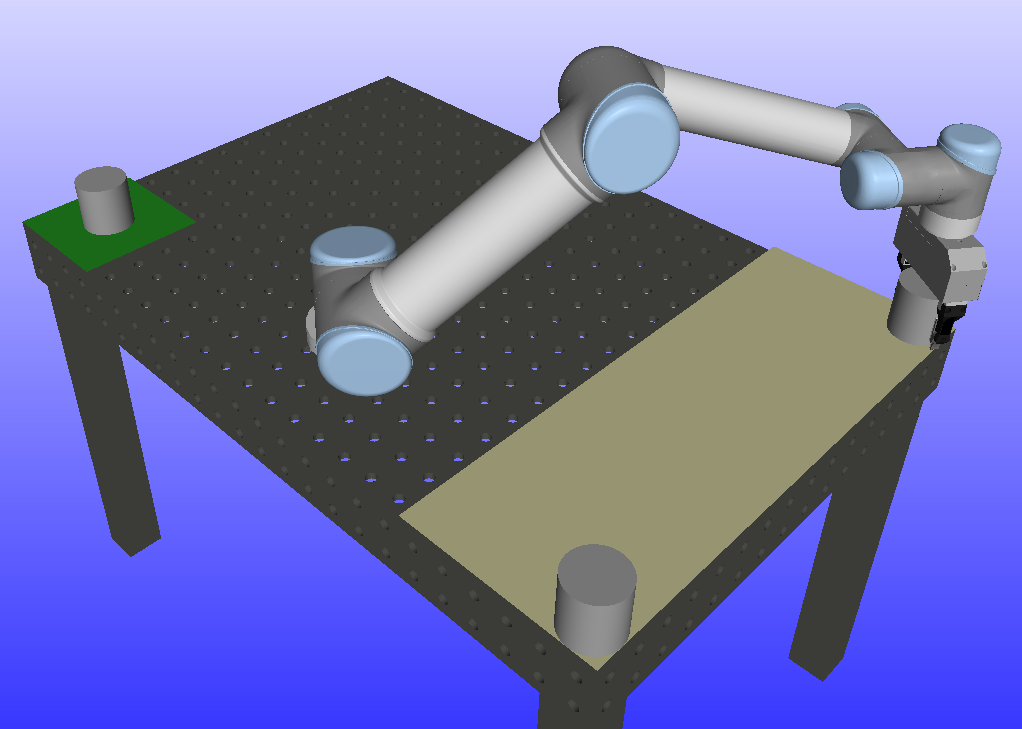
\includegraphics[width=0.9\textwidth]{figures/workcell_setup/final_robot_position1.png}
    \end{subfigure}%
    \begin{subfigure}{0.329\textwidth}
        \centering
        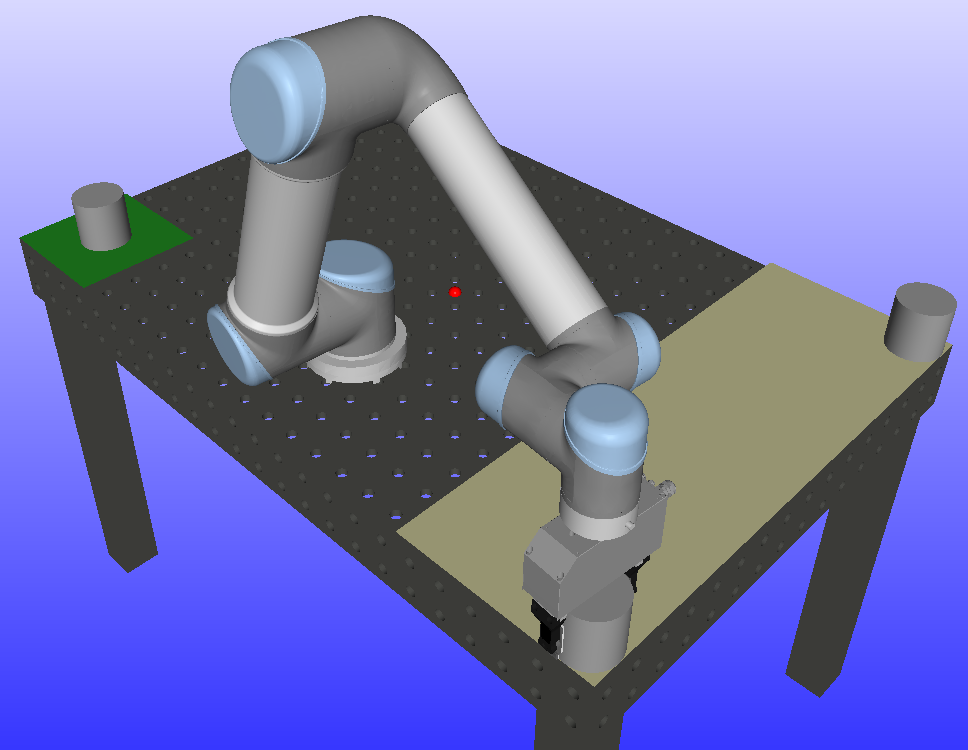
\includegraphics[width=0.9\textwidth]{figures/workcell_setup/final_robot_position2.png}
    \end{subfigure}%
    \begin{subfigure}{0.329\textwidth}
        \centering
        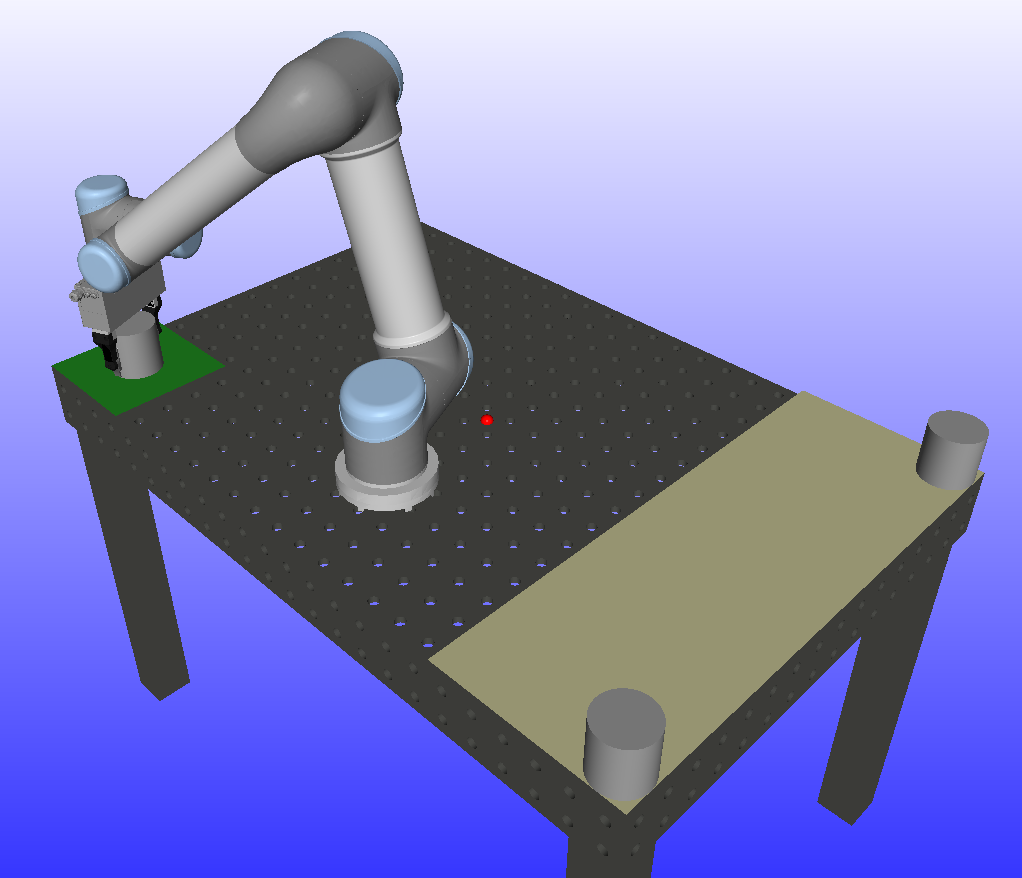
\includegraphics[width=0.9\textwidth]{figures/workcell_setup/final_robot_position3.png}
    \end{subfigure}
    \caption{Illustrations of the robot reachabillity at the position $(0.2, 0.0)$.}
    \label{fig:final_robot_position}
\end{figure}

\subsection{Robot Motion Planning} \label{subsec:robot_motion_planning}
In this section three algorithms for motion planning will be explored. The algorithms are point to point interpolation, point to point interpolation with parabolic blend, and Rapidly-exploring Random Trees Connect, RRT-Connect. The three algorithms will all be analysed on three different configurations, which are shown in Figures \ref{subfig:rrt_cylinder1}, \ref{subfig:rrt_cylinder2} and \ref{subfig:rrt_cylinder3}. The destination of the object is shown in Figure \ref{subfig:rrt_cylinder4}.

\begin{figure}[H]
    \centering
    \begin{subfigure}[t]{0.24\textwidth}
        \centering
        \captionsetup{width=.9\textwidth}
        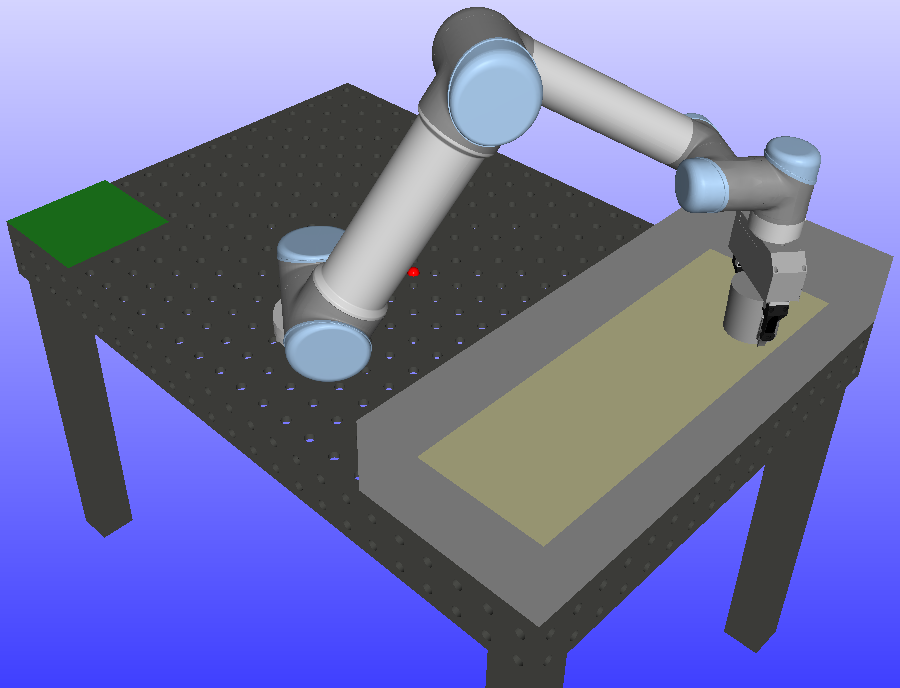
\includegraphics[width=0.9\textwidth]{figures/robot_motion_planning/rrt_connect/cylinder1.png}
        \caption{Cylinder at $(-0.25, 0.474, 0.15)$ with the corresponding robot arm configuration.}
        \label{subfig:rrt_cylinder1}
    \end{subfigure}
    \begin{subfigure}[t]{0.24\textwidth}
        \centering
        \captionsetup{width=.9\textwidth}
        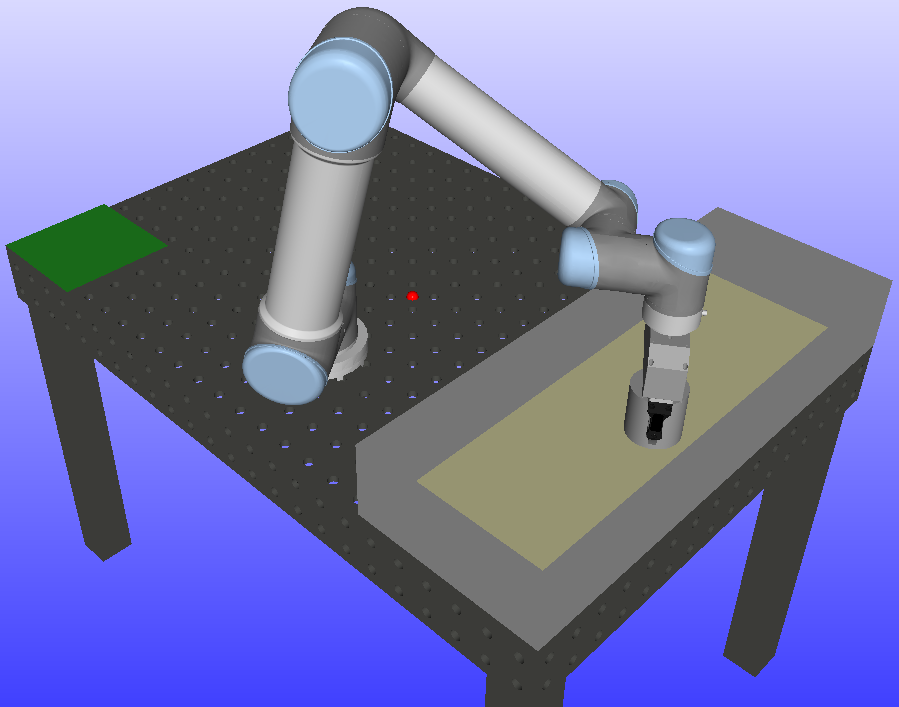
\includegraphics[width=0.9\textwidth]{figures/robot_motion_planning/rrt_connect/cylinder2.png}
        \caption{Cylinder at $(0.0, 0.474, 0.15)$ with the corresponding robot arm configuration.}
        \label{subfig:rrt_cylinder2}
    \end{subfigure}
    \begin{subfigure}[t]{0.24\textwidth}
        \centering
        \captionsetup{width=.9\textwidth}
        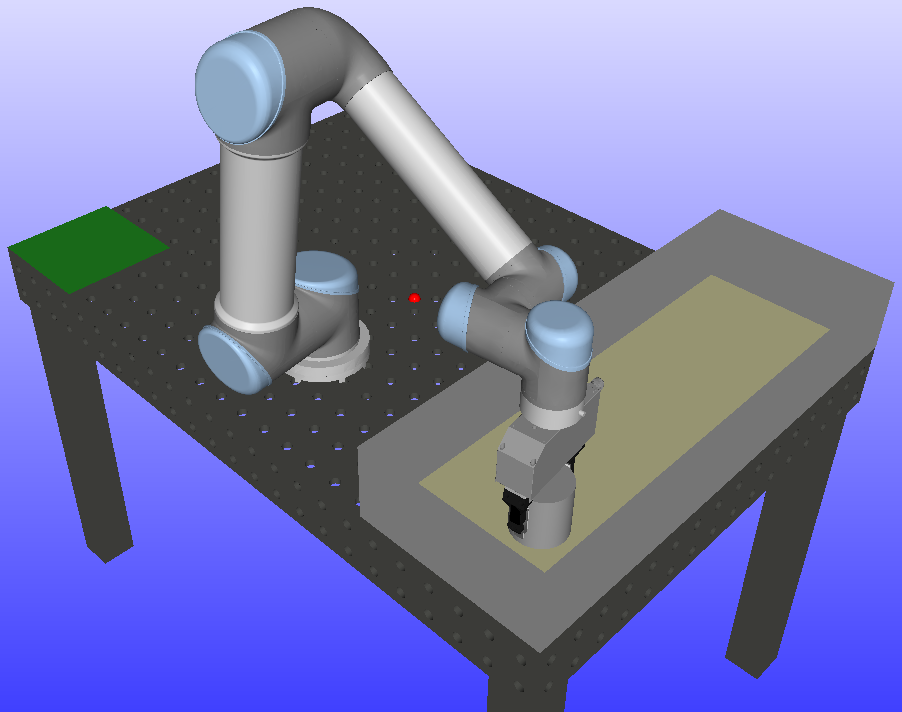
\includegraphics[width=0.9\textwidth]{figures/robot_motion_planning/rrt_connect/cylinder3.png}
        \caption{Cylinder at $(0.25, 0.474, 0.15)$ with the corresponding robot arm configuration.}
        \label{subfig:rrt_cylinder3}
    \end{subfigure}
    \begin{subfigure}[t]{0.24\textwidth}
        \centering
        \captionsetup{width=.9\textwidth}
        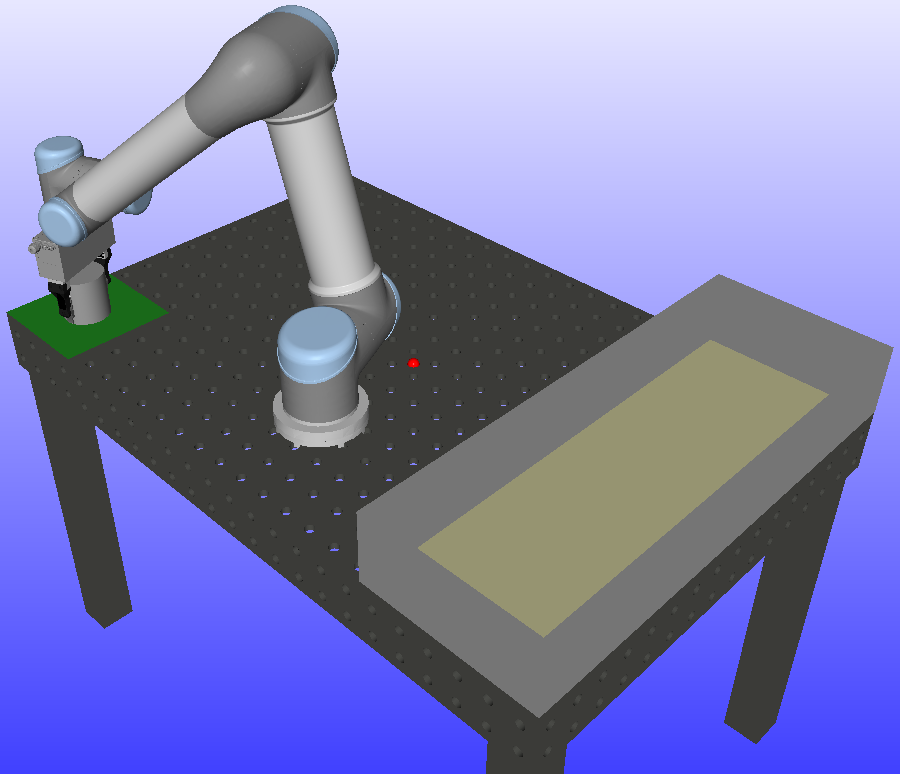
\includegraphics[width=0.9\textwidth]{figures/robot_motion_planning/rrt_connect/cylinder4.png}
        \caption{Final position of the cylinders and the corresponding robot arm configuration.}
        \label{subfig:rrt_cylinder4}
    \end{subfigure}
    \caption{Visualization of the cylinders position on the table and the robot arm configuration to reach the cylinder.}
    \label{fig:rrt_scene}
\end{figure}

In Figure \ref{fig:rrt_scene} the picking area is surrounded by walls, this is only done in Rapidly-exploring Random Trees Connect because otherwise, the algorithm would generate a linear path between the source and the destination. Otherwise, the cylinder positions and the workcell is the same when testing the three methods.

\subsubsection{Point to Point Interpolation} \label{subsec:p2p_interpolation}
When doing interpolation between two points in the workspace there are two options --- Jointspace interpolation and toolspace interpolation. The simplest version is to use jointspace interpolation since no inverse kinematics are required at each calculated point, whereas the toolspace interpolation requires to solve for the joint configurations at each point along the path using inverse kinematics.

A thing to consider when using jointspace interpolation is that it does not have a well defined path for the position and orientation of the end effector between each point since the linearity of the interpolation is for each joint, and not the position and orientation of the end effector. A different approach is the toolspace interpolation. Since the interpolation happens between points that define the position and orientation of the end effector this gives a well defined path for the end effector while the rest of the robot's configuration is decided by solving inverse kinematics. Another thing to consider when doing linear interpolation is that the trajectory is split up at every defined point. This means the robot will stop at every intersection between two parts of the trajectory. A solution to this problem is presented in Section \ref{subsec:p2p_interpolation_parabolic_blend}. For this project, it is chosen to focus on jointspace interpolation.

To do linear interpolation between two points the difference is split up into an evenly distributed number of intermediate points. To calculate the fraction of time between each point, resulting in a linear velocity, Equation \ref{eq:timestep} is used.
\begin{equation}\label{eq:timestep}
    s(t)=\frac{t-t_{i-1}}{t_i-t_{i-1}}
\end{equation}
To calculate the next point for the interpolation the difference between the start and end points times the fraction of time is added to the start point. The equation used is from \cite{lec_notes} and is seen in Equation \ref{eq:linear_int}
\begin{equation}\label{eq:linear_int}
    X(s(t))=X_{i-1}+(X_i-X_{i-1})s(t)\quad0<=s<=1
\end{equation}
The configurations used to interpolate between are seen in Figure \ref{fig:interpolation_points}.

\begin{figure}[H]
    \centering
    \begin{subfigure}[t]{0.3\textwidth}
        \centering
        \captionsetup{width=.9\textwidth}
        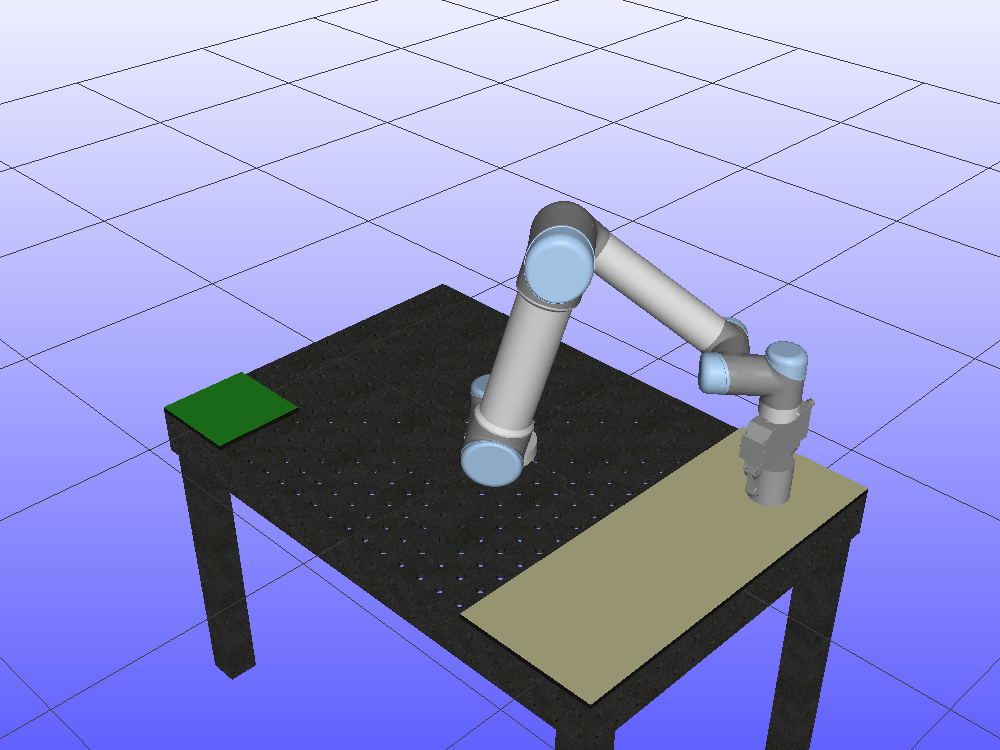
\includegraphics[width=0.9\textwidth]{figures/p2p_interpolation/on_pick.png}
        \caption{Place}
        \label{}
    \end{subfigure}
    \begin{subfigure}[t]{0.3\textwidth}
        \centering
        \captionsetup{width=.9\textwidth}
        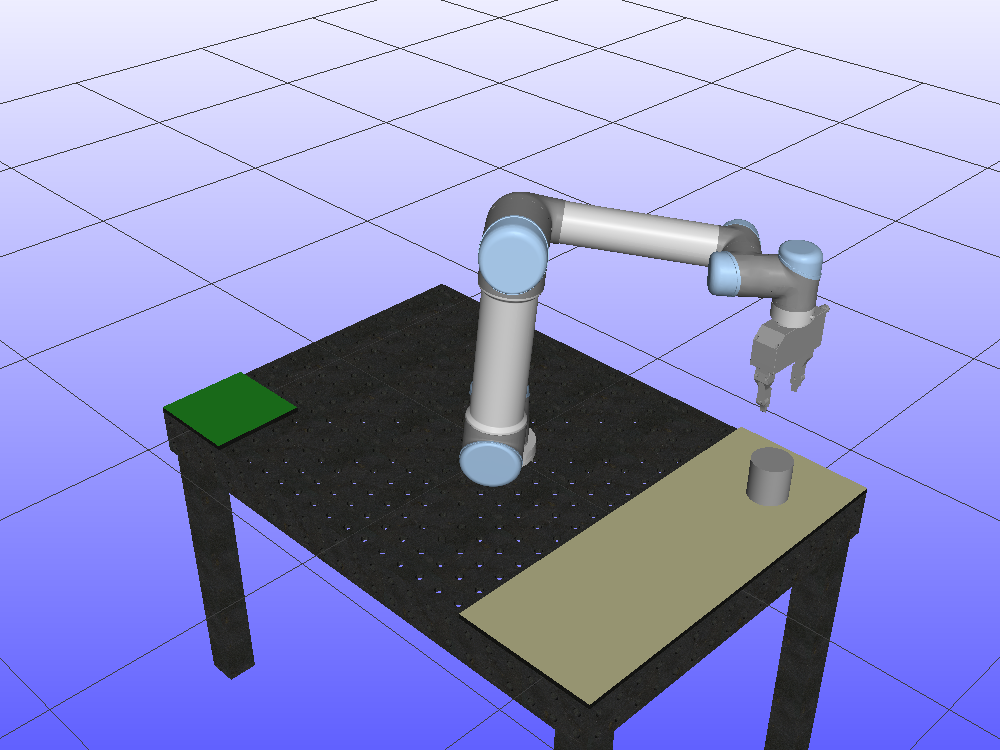
\includegraphics[width=0.9\textwidth]{figures/p2p_interpolation/above_pick.png}
        \caption{Above place}
        \label{}
    \end{subfigure}
    \begin{subfigure}[t]{0.3\textwidth}
        \centering
        \captionsetup{width=.9\textwidth}
        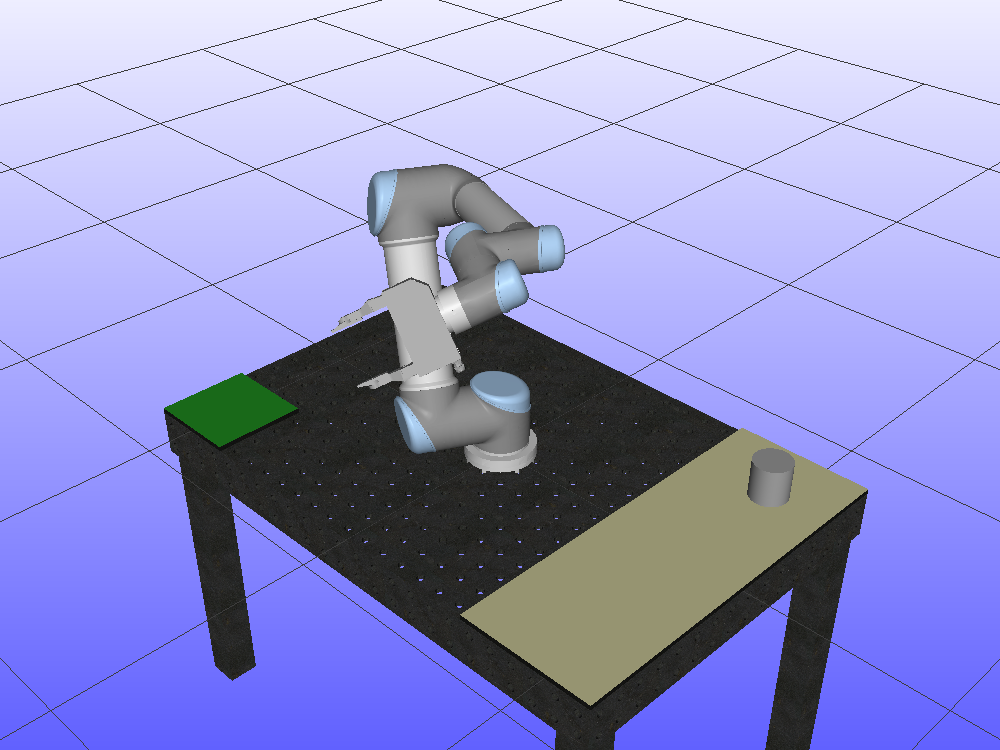
\includegraphics[width=0.9\textwidth]{figures/p2p_interpolation/intermediate1.png}
        \caption{Intermediate point 1}
        \label{}
    \end{subfigure}
    \begin{subfigure}[t]{0.3\textwidth}
        \centering
        \captionsetup{width=.9\textwidth}
        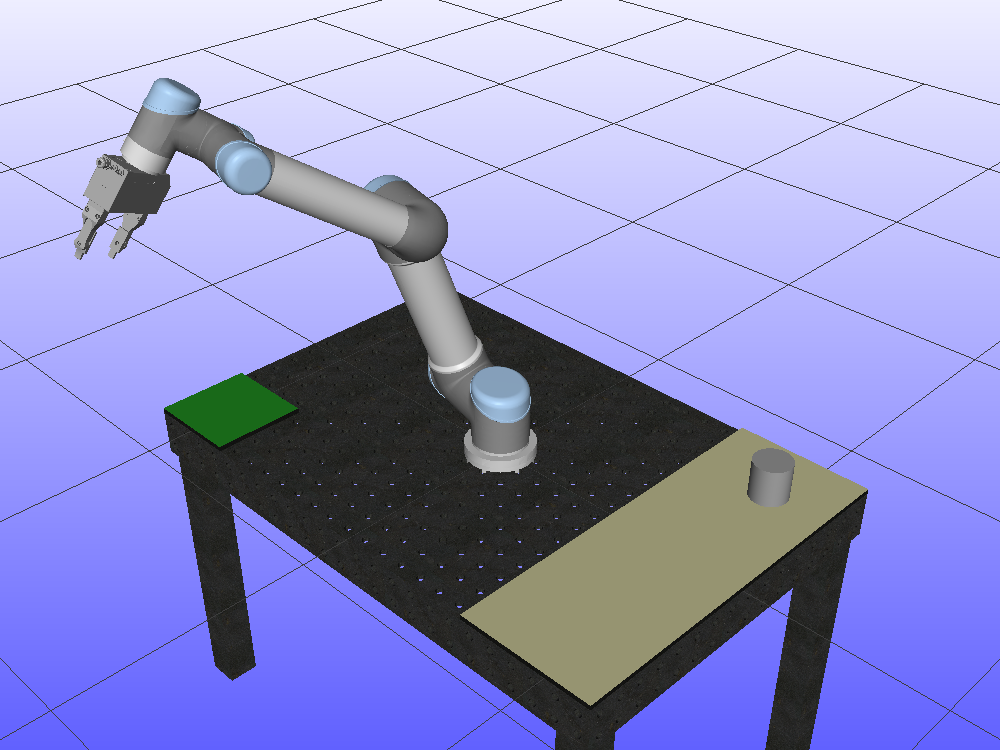
\includegraphics[width=0.9\textwidth]{figures/p2p_interpolation/intermediate2.png}
        \caption{Intermediate point 2}
        \label{}
    \end{subfigure}
    \begin{subfigure}[t]{0.3\textwidth}
        \centering
        \captionsetup{width=.9\textwidth}
        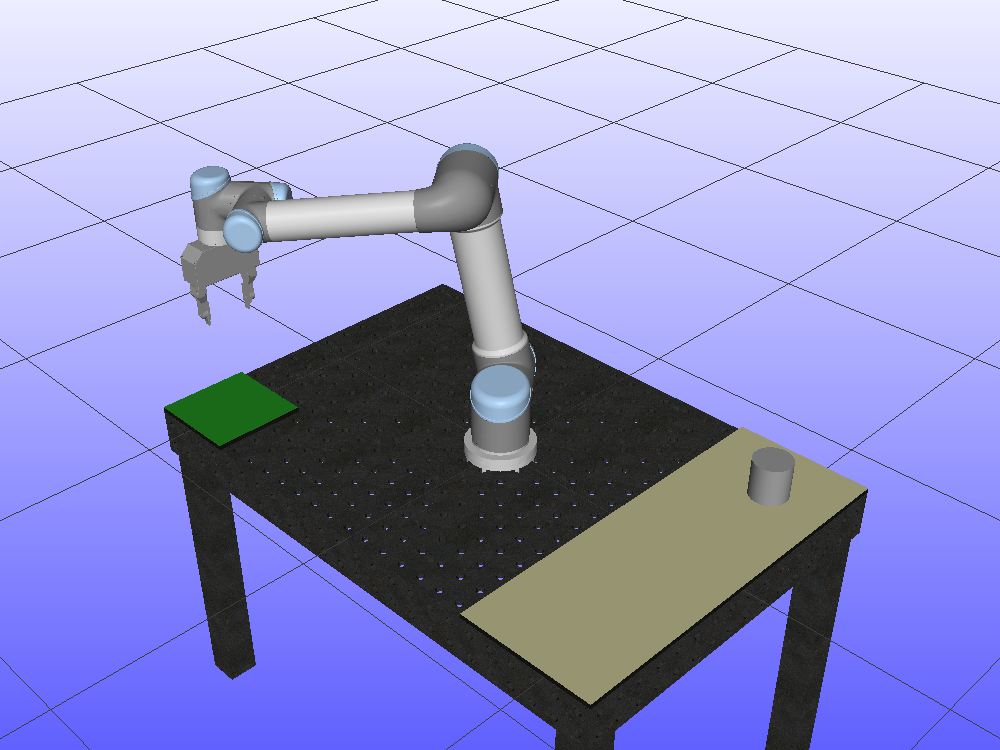
\includegraphics[width=0.9\textwidth]{figures/p2p_interpolation/above_place.png}
        \caption{Above place}
        \label{}
    \end{subfigure}
    \begin{subfigure}[t]{0.3\textwidth}
        \centering
        \captionsetup{width=.9\textwidth}
        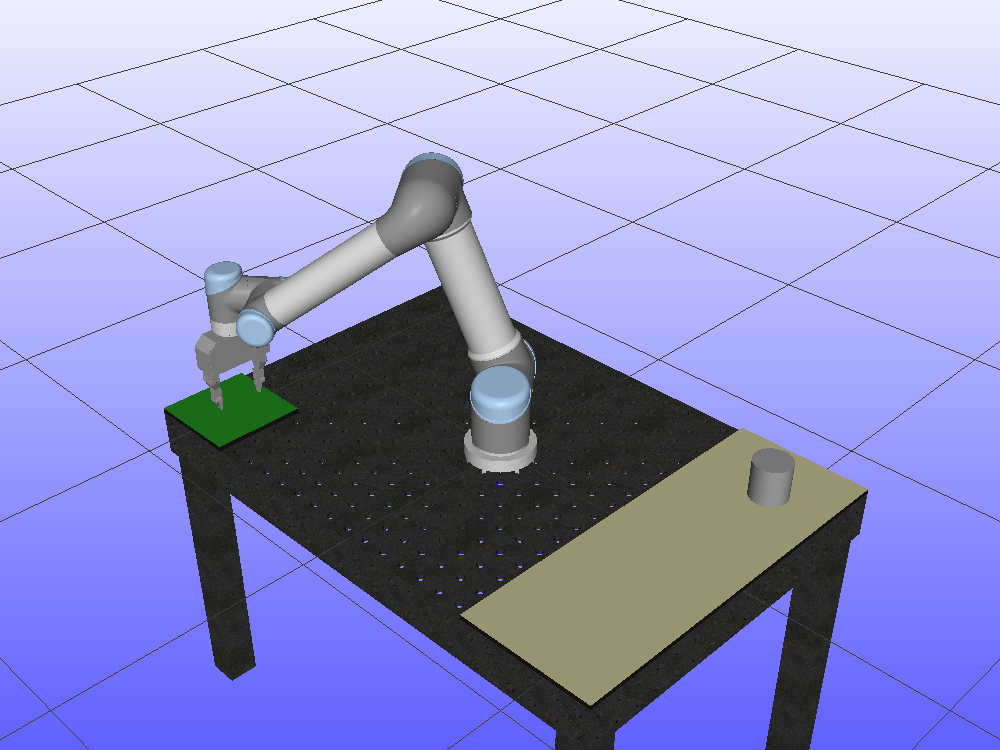
\includegraphics[width=0.9\textwidth]{figures/p2p_interpolation/on_place.png}
        \caption{Place}
        \label{}
    \end{subfigure}
    \caption{Points used to interpolate between.}
    \label{fig:interpolation_points}
\end{figure}
In Figure \ref{fig:p2p_int} the resulting path is seen plotted. The circles indicate the points specified to blend between and the lines are the resulting configurations for the end effector relative to the robot's base frame. Here it is seen that interpolating in jointspace does not result in straight lines for the end effector. If the interpolation was done in toolspace the expected result would be straight lines between the defined configurations.
\begin{figure}[h]
    \centering
    \begin{subfigure}[t]{0.45\textwidth}
        \centering
        \captionsetup{width=.9\textwidth}
        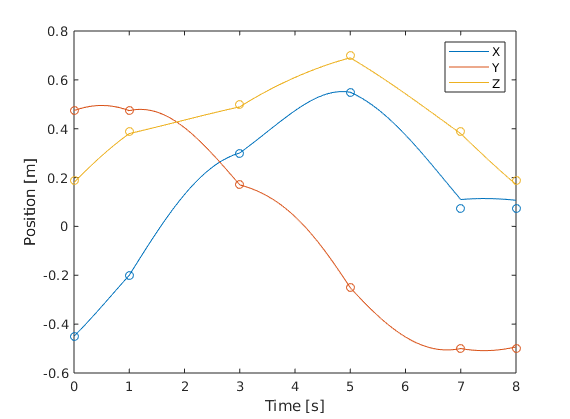
\includegraphics[width=0.9\textwidth]{figures/p2p_interpolation/d_joint_space_int_without_blend_position.png}
        \caption{The position of the end effector in the robot's base frame.}
        \label{}
    \end{subfigure}
    \begin{subfigure}[t]{0.45\textwidth}
        \centering
        \captionsetup{width=.9\textwidth}
        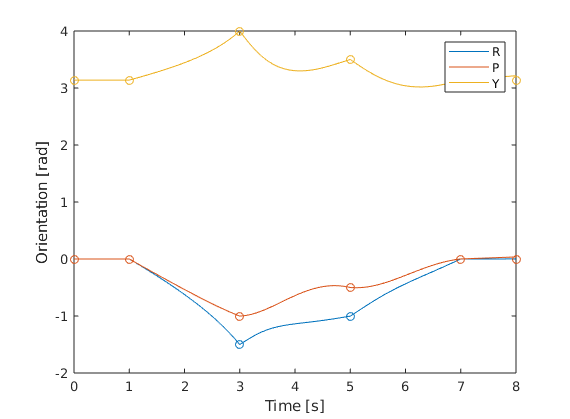
\includegraphics[width=0.9\textwidth]{figures/p2p_interpolation/d_joint_space_int_without_blend_orientation.png}
        \caption{The orientation of the end effector.}
        \label{}
    \end{subfigure}
    \caption{The resulting trajectory for the end effector when interpolating in jointspace.}
    \label{fig:p2p_int}
\end{figure}

\subsubsection{Point to Point Interpolation with Parabolic Blend} \label{subsec:p2p_interpolation_parabolic_blend}
As seen in Section \ref{subsec:p2p_interpolation} one downside to linear point to point interpolation is the lack of smooth motion at each point. To combat the quick changes in velocity and hard changes in direction at each point a parabolic blend can be implemented around each point. This creates a smooth transition between the two interpolated linear segments, both for velocity and position.

The resulting path using point to point interpolation with parabolic blends in jointspace is seen in Figure \ref{fig:p2p_int_blend}. As for the path without parabolic blends, the circles indicate the specified configurations to move between. Here it is seen that the segments transition smoothly at every defined point rather than having a sharp turn directly on the point.

\begin{figure}[H]
    \centering
    \begin{subfigure}[t]{0.45\textwidth}
        \centering
        \captionsetup{width=.9\textwidth}
        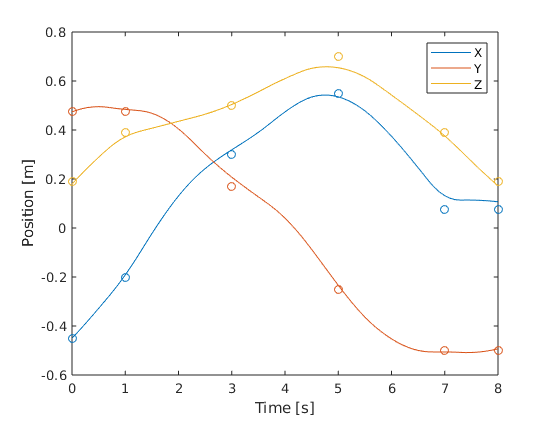
\includegraphics[width=0.9\textwidth]{figures/p2p_interpolation/d_joint_space_int_with_blend_position.png}
        \caption{The position of the end effector in the robot's base frame.}
        \label{}
    \end{subfigure}
    \begin{subfigure}[t]{0.45\textwidth}
        \centering
        \captionsetup{width=.9\textwidth}
        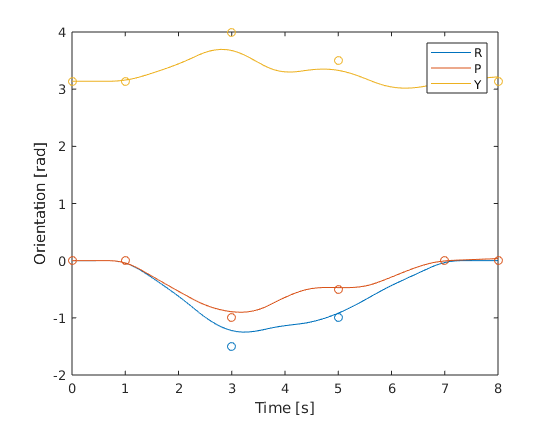
\includegraphics[width=0.9\textwidth]{figures/p2p_interpolation/d_joint_space_int_with_blend_orientation.png}
        \caption{The orientation of the end effector.}
        \label{}
    \end{subfigure}
    \caption{The resulting trajectory for the end effector when interpolating with parabolic blends in jointspace.}
    \label{fig:p2p_int_blend}
\end{figure}

The parabolic blend uses Equation \ref{eq:parabolic_blend} from \cite{lec_notes}.
\begin{equation}\label{eq:parabolic_blend}
    P(t-T,X,v_1,v_2,\tau)=\frac{v_2-v_1}{4\tau}(t-T+\tau)^2+v_1(t-T)+X
\end{equation}
Given three points, $v_1$ and $v_2$ are the velocities for the segment between the first and second and second and third points respectively. X is the configuration and T is the time at the middle point. $\tau$ is the blend time on either side of the middle point --- hence the total blend time ends up as $2\cdot\tau$ and it is centered around T. To generate a path with multiple points to blend between it was chosen to have $\tau$ be $\frac{1}{3}$ of the shortest segment near the point. This way it is avoided that any blends overlap and leaves at least $\frac{1}{3}$ linear path in the middle.

\subsubsection{Rapidly-exploring Random Trees Connect} \label{subsec:rrt_connect}
In this section, the motion planning algorithm RRT-Connect is explored for performing a pick and place action in the scene shown in Figure \ref{fig:rrt_scene}. The RRT-Connect algorithm is introduced in the paper \cite{rrt_connect} for motion planning in high-dimensional spaces. RRT-Connect varies from RRT by growing two trees, one from the source and one from the destination, and the trees grow towards each other by the use of a connect heuristic.

To estimate the best step size for RRT-Connect various step sizes are analysed for the 3 positions in Figure \ref{fig:rrt_scene}. The parameters considered are the planning time, the number of nodes and the path length. In Figures \ref{fig:rrt_cylinder_25}, \ref{fig:rrt_cylinder_0} and \ref{fig:rrt_cylinder_-25} the results of the analyses are shown.
\begin{figure}[H]
    \centering
    \noindent\makebox[\textwidth]{%
    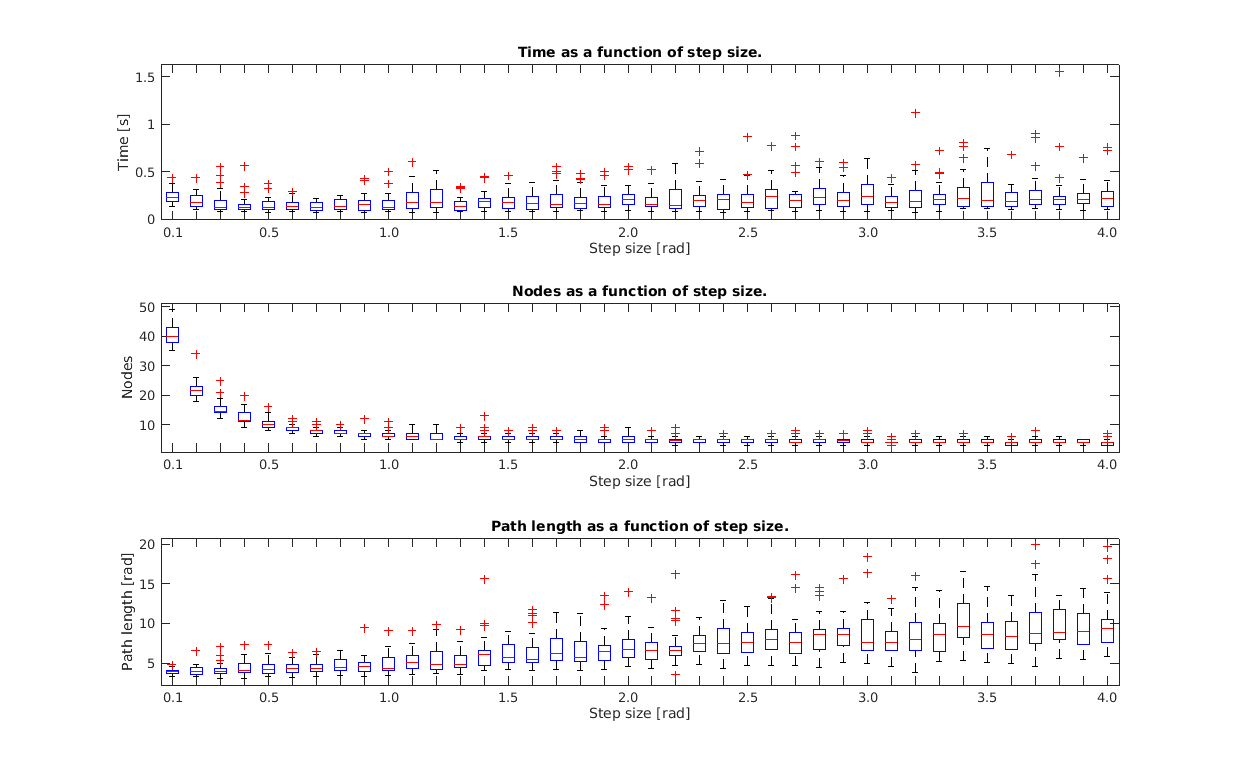
\includegraphics[width=1.2\textwidth]{figures/robot_motion_planning/rrt_connect/cylinder_25.png}}
    \caption{RRT-Connect with the cylinder at (0.25, 0.474, 0.15).}
    \label{fig:rrt_cylinder_25}
\end{figure}
\begin{figure}[H]
    \centering
    \noindent\makebox[\textwidth]{%
    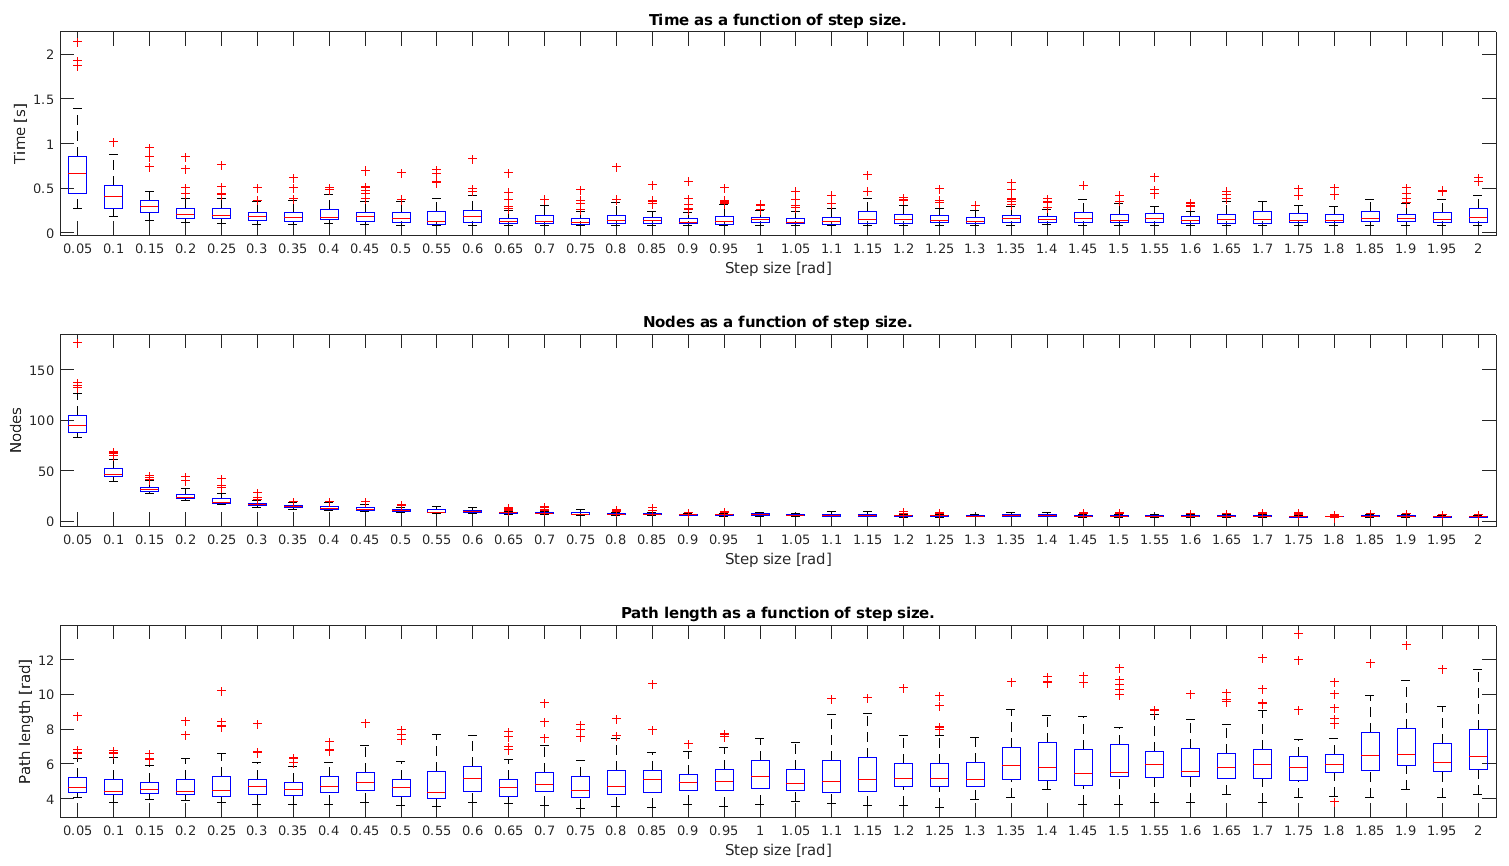
\includegraphics[width=1.2\textwidth]{figures/robot_motion_planning/rrt_connect/cylinder_0.png}}
    \caption{RRT-Connect with the cylinder at (0.0, 0.474, 0.15).}
    \label{fig:rrt_cylinder_0}
\end{figure}
\begin{figure}[H]
    \centering
    \noindent\makebox[\textwidth]{%
    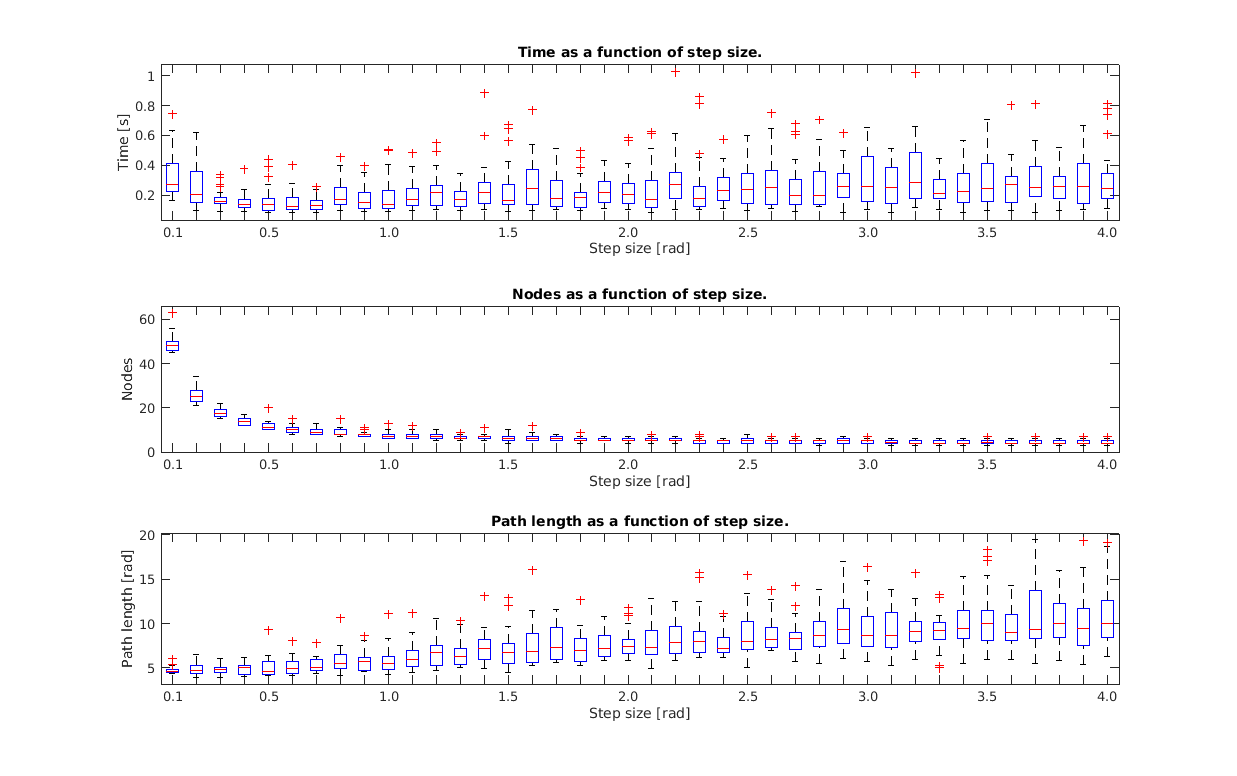
\includegraphics[width=1.2\textwidth]{figures/robot_motion_planning/rrt_connect/cylinder_-25.png}}
    \caption{RRT-Connect with the cylinder at (-0.25, 0.474, 0.15).}
    \label{fig:rrt_cylinder_-25}
\end{figure}
From the Figures \ref{fig:rrt_cylinder_25}, \ref{fig:rrt_cylinder_0} and \ref{fig:rrt_cylinder_-25}, the step size of RRT-Connect is chosen to $0.6$. This step size is deemed acceptable in time, number of nodes and path length for all 3 positions of the cylinder. The results of RRT-Connect with a step size of $0.6$ are shown in Table \ref{tab:rrt_connect_0.6}.
\begin{table}[H]
\centering
\resizebox{\textwidth}{!}{%
\begin{tabular}{llll}
\toprule
\textbf{RRT-Connect} & \textbf{Planning time [s]} & \textbf{Path length [rad]} & \textbf{Number of nodes} \\ \midrule
Cylinder in position (0.25, 0.474) & $0.1307(\pm 0.0387)$ & $4.4025(\pm 0.7935)$ & $8.9(\pm 1.2817)$ \\
Cylinder in position (0, 0.474) & $0.2126(\pm 0.1304)$ & $5.1726(\pm 0.8953)$ & $10.08 (\pm 1.5497)$ \\
Cylinder in position (-0.25, 0.474) & $0.1578(\pm 0.0537)$ & $5.1016(\pm 0.5578)$ & $10.04 (\pm 0.9889)$ \\ \bottomrule
\end{tabular}%
}
\caption{The results of the RRT-Connect with a step size of $0.6$}
\label{tab:rrt_connect_0.6}
\end{table}

\subsubsection{Comparison of the Robot Motion Planning Methods Implemented} \label{subsubsec:comparision_robotics}
To compare the three robot motion planning methods the planning time and the path length of each method is considered. Table \ref{tab:cyl1_compare} shows the planning time and path length for each method with the cylinder at different positions.
\begin{table}[H]
\centering
\resizebox{\textwidth}{!}{%
\begin{tabular}{lll}
\toprule
\textbf{Method --- Cylinder in position (0.25, 0.474)} & \textbf{Planning time [s]} & \textbf{Path length [rad]} \\ \midrule
Point to Point Interpolation & 
$2\cdot10^{-5}(\pm1.4142\cdot10^{-4})$ & $8.1819(\pm1.7944\cdot10^{-15})$ \\
Point to Point Interpolation with Parabolic Blend & 
$4\cdot10^{-5}(\pm1.9795\cdot10^{-4})$ & $7.6840(\pm8.9720\cdot10^{-15})$ \\
Rapidly-exploring Random Trees Connect & $0.1307\ (\pm\ 0.0387)$ & $4.4025\ (\pm\     0.7935)$ \\ \midrule
\textbf{Method --- Cylinder in position (0.0, 0.474)} & \textbf{Planning time [s]} & \textbf{Path length [rad]} \\ \midrule
Point to Point Interpolation & 
$2\cdot10^{-5}(\pm1.4142\cdot10^{-4})$ & $8.0742(\pm7.1776\cdot10^{-15})$ \\
Point to Point Interpolation with Parabolic Blend & 
$6\cdot10^{-5}(\pm2.3990\cdot10^{-4})$ & $7.5544(\pm3.5888\cdot10^{-15})$ \\
Rapidly-exploring Random Trees Connect & $0.2126\ (\pm\ 0.1304)$ & $5.1726\ (\pm\ 0.8953)$ \\ \midrule
\textbf{Method --- Cylinder in position (-0.25, 0.474)} & \textbf{Planning time [s]} & \textbf{Path length [rad]} \\ \midrule
Point to Point Interpolation & 
$2\cdot10^{-5}(\pm1.4142\cdot10^{-4})$ & $8.4105(\pm7.1776\cdot10^{-15})$ \\
Point to Point Interpolation with Parabolic Blend & 
$6\cdot10^{-5}(\pm2.3990\cdot10^{-4})$ & $7.8404(\pm8.9720\cdot10^{-15})$ \\
Rapidly-exploring Random Trees Connect & $0.1578\ (\pm\ 0.0537)$ & $5.1016\ (\pm\ 0.5578)$ \\ \bottomrule
\end{tabular}%
}
\caption{Summary of the planning time and path length for the three implemented methods.}
\label{tab:cyl1_compare}
\end{table}
From Table \ref{tab:cyl1_compare}, the RRT-Connect method has the longest planning time and the shortest path length. However, the standard deviation is much higher than the other methods, which is because the method is random. The downside of RRT-Connect, when compared to the other methods, is that point to point interpolation with and without parabolic blend has some predefined path configurations. The predefined configurations are protected from singularities by the developer, thus making these methods more secure. 

For further comparison of the three methods the TCP displacement is shown in Figure \ref{fig:comp_tcp}, when executing from the object configurations to the goal configurations with the object attached to the TCP. 
\begin{figure}[H]
    \centering
    \begin{subfigure}[t]{0.49\textwidth}
        \centering
        \captionsetup{width=.9\textwidth}
        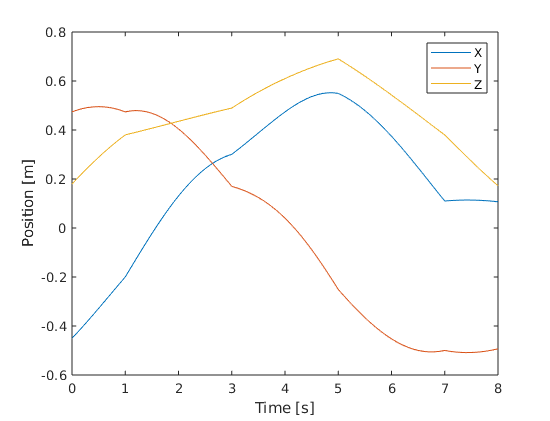
\includegraphics[width=0.9\textwidth]{figures/p2p_interpolation/joint_space_int_without_blend_position.png}
        \caption{Point to point interpolation x, y and z displacement of the TCP from object to goal.}
        \label{subfig:p2p_xyz}
    \end{subfigure}
    \begin{subfigure}[t]{0.49\textwidth}
        \centering
        \captionsetup{width=.9\textwidth}
        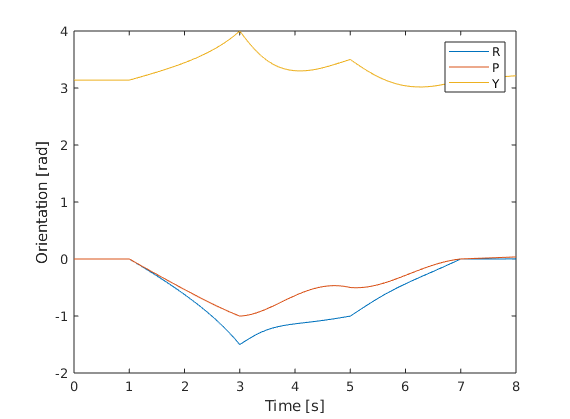
\includegraphics[width=0.93\textwidth]{figures/p2p_interpolation/joint_space_int_without_blend_orientation.png}
        \caption{Point to point interpolation roll, pitch and yaw displacement of the TCP from object to goal.}
        \label{subfig:p2p_rpy}
    \end{subfigure}
    \begin{subfigure}[t]{0.49\textwidth}
        \centering
        \captionsetup{width=.9\textwidth}
        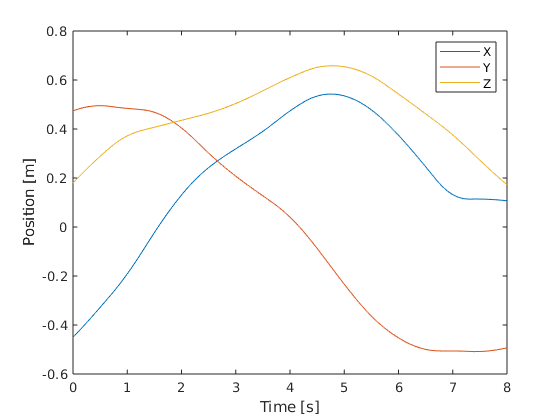
\includegraphics[width=0.9\textwidth]{figures/p2p_interpolation/joint_space_int_with_blend_position.png}
        \caption{Point to point interpolation with parabolic blend x, y and z displacement of the TCP from object to goal.}
        \label{subfig:p2p_parabolic_xyz}
    \end{subfigure}
    \begin{subfigure}[t]{0.49\textwidth}
        \centering
        \captionsetup{width=.9\textwidth}
        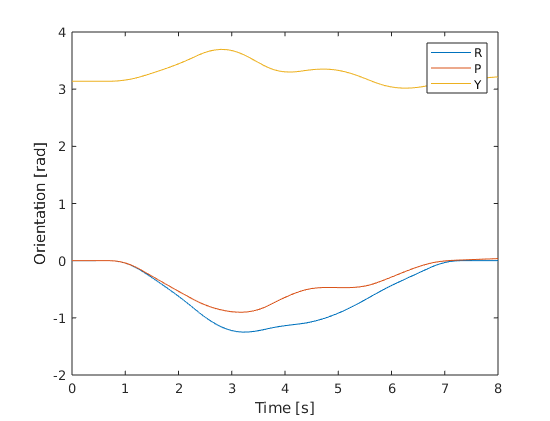
\includegraphics[width=0.9\textwidth]{figures/p2p_interpolation/joint_space_int_with_blend_orientation.png}
        \caption{Point to point interpolation with parabolic blend roll, pitch and yaw displacement of the TCP from object to goal.}
        \label{subfig:p2p_parabolic_rpy}
    \end{subfigure}
    \begin{subfigure}[t]{0.49\textwidth}
        \centering
        \captionsetup{width=.9\textwidth}
        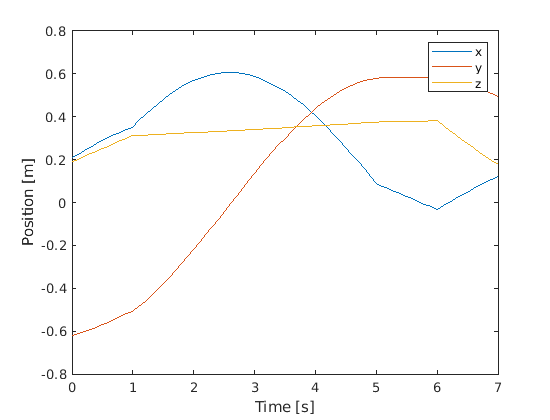
\includegraphics[width=0.9\textwidth]{figures/robot_motion_planning/rrt_connect/xyz.png}
        \caption{Rapidly-exploring Random Trees Connect x, y and z displacement of the TCP from object to goal.}
        \label{subfig:rrt_xyz}
    \end{subfigure}
    \begin{subfigure}[t]{0.49\textwidth}
        \centering
        \captionsetup{width=0.9\textwidth}
        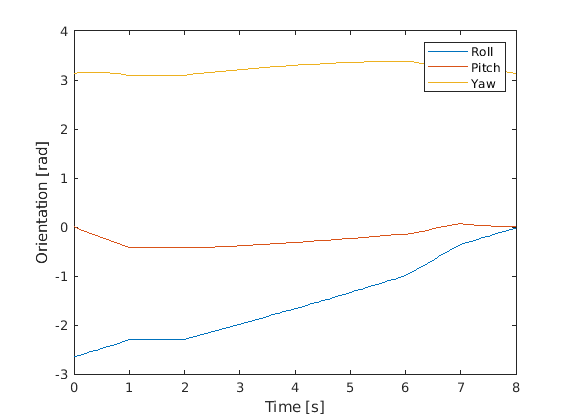
\includegraphics[width=0.9\textwidth]{figures/robot_motion_planning/rrt_connect/rpy.png}
        \caption{Rapidly-exploring Random Trees Connect roll, pitch and yaw displacement of the TCP from object to goal.}
        \label{subfig::rrt_xyz}
    \end{subfigure}
    \caption{Comparison of TCP displacement when executing from object at position $(0.25, 0.474)$ to goal with the object attached.}
    \label{fig:comp_tcp}
\end{figure}

From Figures \ref{subfig:p2p_parabolic_xyz} and \ref{subfig:p2p_parabolic_rpy}, it is seen that the point to point interpolation with parabolic blend moves more smoothly than point to point interpolation, shown in Figures \ref{subfig:p2p_xyz} and \ref{subfig:p2p_rpy}, which is expected.

\begin{figure}[H]
    \centering
    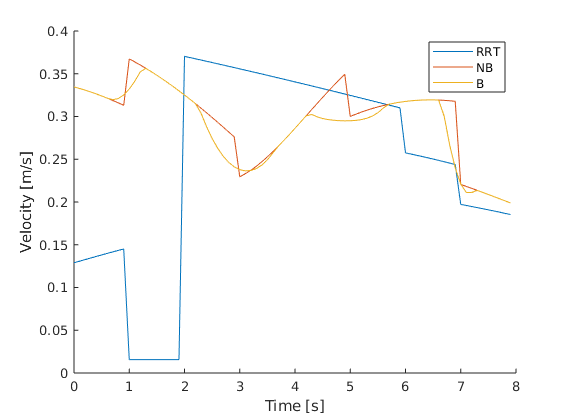
\includegraphics[width=.5\textwidth]{figures/robot_motion_planning/Tool_velocity.png}
    \caption{Velocity in 3D space for the tool point. \textit{RRT:} RRT-Connect, \textit{NB:} Point to point interpolation, \textit{B:} Point to point interpolation with parabolic blend.}
    \label{fig:tool_3d_velocity}
\end{figure}

Figure \ref{fig:tool_3d_velocity}, shows the velocity profile for the tool point of the robot when moving from the object to the goal with the object attached. The velocity profile for point to point interpolation and point to point interpolation with blend are both based on the same set of points and hence give the same profile with the blended trajectory having smooth transitions in velocity. The RRT-Connect velocity profile is based on a path found using RRT-Connect and then linear interpolation between each segment. The reason for the very low velocity between one and two seconds in Figure \ref{fig:tool_3d_velocity} is that RRT-Connect has found two points relatively close together and the implementation of the linear interpolation, for now, only supports integer values for the time for each segment.

\end{document}